\subsection{Mapping CML to Other Modeling Notations}\label{subsec:mapping}

Part of the CML metamodel (presented in section \ref{subsec:metamodel}) may be considered a small subset of the UML  \cite{uml} metamodel.
Thus, the structural (static) elements of CML models can be transformed into UML class diagrams. The example CML model in the listing of figure \ref{fig:store} is mapped to the UML model in figure \ref{fig:uml}.

\begin{figure}
\centering
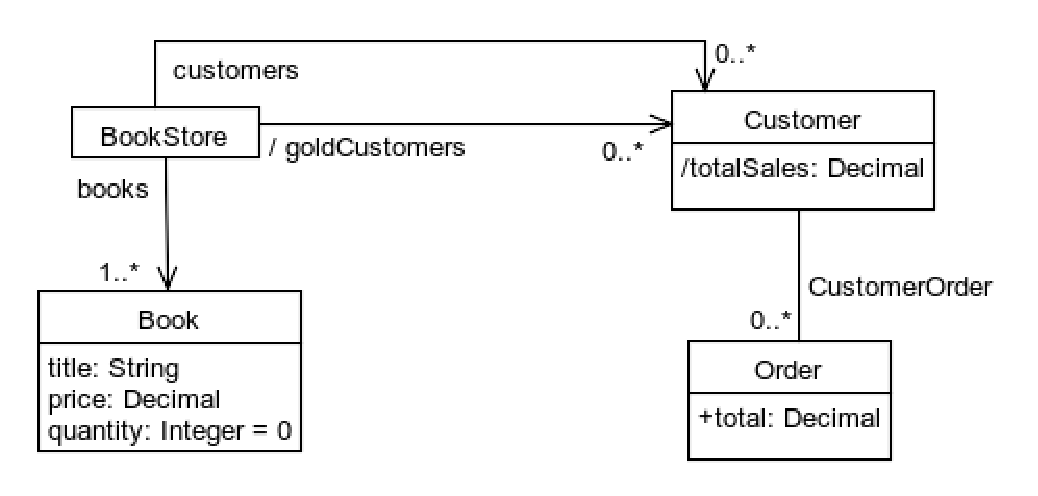
\includegraphics[width=0.8\textwidth]{language/diagram-uml}
\caption{The class diagram representing in UML  \cite{uml} the same CML model listed in figure \ref{fig:store}.}
\label{fig:uml}
\end{figure}

In the UML class diagram of figure \ref{fig:uml}:
\begin{itemize}
\item the CML concepts (\emph{BookStore}, \emph{Book}, \emph{Customer} and \emph{Order}) are mapped to corresponding UML classes;
\item the CML properties that represent unidirectional associations
(\emph{books}, \emph{customers}, and \emph{goldCustomers} of \emph{BookStore})
are mapped to UML associations with corresponding roles
(showing the navigability direction, and matching the property names);
\item the CML bidirectional association \emph{CustomerOrder}
(comprised by two CML properties: \emph{Customer.orders} and \emph{Order.customer})
is mapped to a UML association with bidirectional navigability (no direction arrow).
\end{itemize}

As demonstrated by this example,
CML strives to enable modeling at the same conceptual level as allowed by UML.
When compared to the UML metamodel,
the CML metamodel supports only a core set of its elements (as shown in subsection \ref{subsec:metamodel}).
This minimally viable core has been intentionally designed to validate CML's objectives.



 